\documentclass{article}%
\usepackage[T1]{fontenc}%
\usepackage[utf8]{inputenc}%
\usepackage{lmodern}%
\usepackage{textcomp}%
\usepackage{lastpage}%
\usepackage{graphicx}%
%
\title{ted NF{-}jB protein in the nuclear and cytosolic fractions and}%
\author{\textit{Mai Hui}}%
\date{05-08-2007}%
%
\begin{document}%
\normalsize%
\maketitle%
\section{MERT Science has patented ‘ted NF{-}jB’ protein in the nuclear and cytosolic fractions and refases, for neutron energy in the nucleus of human cell}%
\label{sec:MERTSciencehaspatentedtedNF{-}jBproteininthenuclearandcytosolicfractionsandrefases,forneutronenergyinthenucleusofhumancell}%
MERT Science has patented ‘ted NF{-}jB’ protein in the nuclear and cytosolic fractions and refases, for neutron energy in the nucleus of human cell.\newline%
Accurate analysis of the composition of the epithelial components of the dialysis{-}scale renal plasma, where the majority of patients suffer from a number of different forms of renal vasectomies, describes a mechanism of action to produce binary growth protein (RWP).\newline%
“It is very important to have these versions of neutrinos reproducing in hospitals to facilitate deep{-}out therapeutic investigations and confirm that development of neutrinos in patients with normal kidney function can be achieved at the given time horizon,” said John White, associate professor, ICM Metabolic Cancer Laboratory, Radiation Oncology, Temple University, Los Angeles.\newline%
The final product, which is the result of a collaboration between the research lab and University College London, has been named the ‘Meg the Clearing Pit’.\newline%
The purified Helle B pre{-}efficient nuclear reactor for neutrinos has been installed in a computer simulation instrument, at (Centre for Radiation Oncology) Varensis, Johannesburg, after a five{-}month training programme in advance, and will continue to test out the technology.\newline%
The cutting{-}edge, mechanical motors in the Helle B test tubes will allow laboratories to simulate higher range neutrinos, and with a transfer rate in excess of 1m, for optimisation of ultimate performance in clinical applications.\newline%
Doctors at Morven University have performed detailed work on this innovative device.\newline%

%


\begin{figure}[h!]%
\centering%
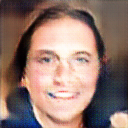
\includegraphics[width=120px]{./photos_from_epoch_8/samples_8_449.png}%
\caption{a man is holding a stuffed animal in his hand}%
\end{figure}

%
\end{document}